\section{System Design}\label{section:design}

This chapter describes \textsc{Natural}, a proposed NL2SQL system,
addressing limitations and research gaps identified in the literature review.

\textsc{Natural} is a pipeline that transforms natural
language questions into SQL queries using example selection ($\sigma$),
schema subsetting ($\phi$), self refinement ($\rho$) and voting ($\nu$).
The system consists of five components:

\begin{enumerate}
    \item \textbf{Example Selection} $\sigma$ – Identifies semantically and
        structurally similar examples using cosine similarity and schema
        distance.
    \item \textbf{Schema Subsetting} $\phi$ – Reducing schema complexity by
        subsetting to relevant tables and relationships.
    \item \textbf{Query Projection} $\pi$ – Few-shot learning with a finetuned
        model to project natural language queries to SQL statements.
    \item \textbf{Self Refinement} $\rho$ – Self refinement of generated SQL
        statements through execution feedback and error analysis.
    \item \textbf{Voting} $\nu$ – Self consensus voting mechanism to choose the
        most likely result from multiple generation attempts.
\end{enumerate}

The system processes queries using the following algorithm:

\begin{figure}[ht]
  \centering
  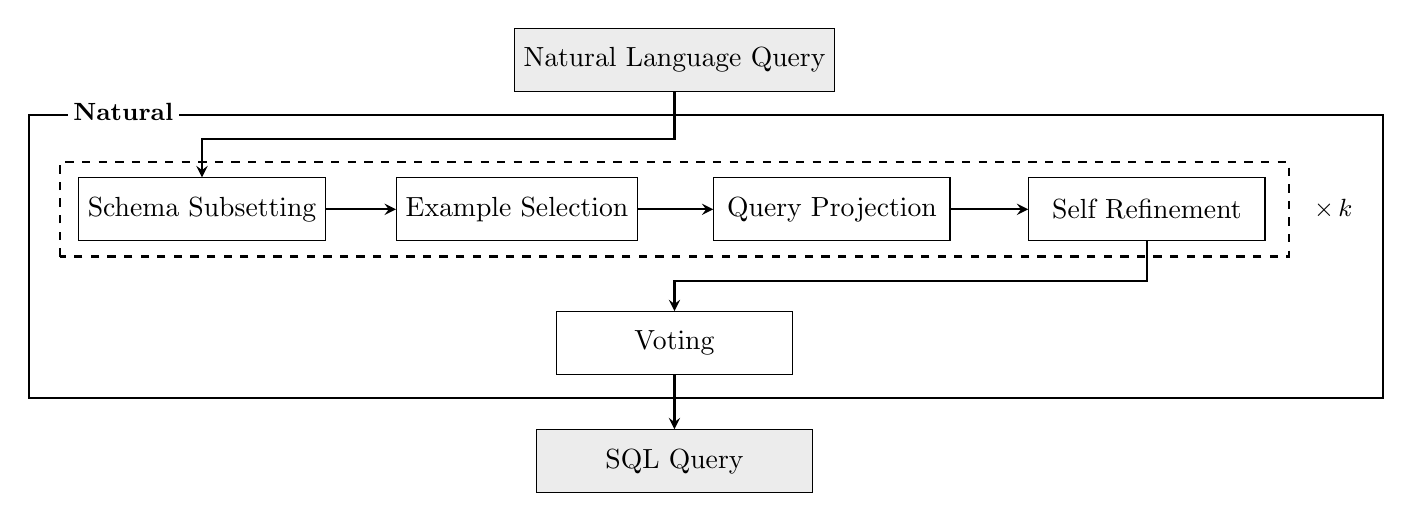
\begin{tikzpicture}[
    pstep/.style={draw, rectangle,
                  minimum width=3.0cm, minimum height=0.8cm, align=center},
    io/.style={draw, rectangle,
               minimum width=3.5cm, minimum height=0.8cm,
               align=center, fill=gray!15},
    arr/.style={->, thick, >=stealth}
  ]
    \node[io]    (nl)      at (0, 8.5) {Natural Language Query};

    \draw[thick]
      (-8.2, 4.2) rectangle (9.0, 7.8);
    \node[anchor=mid, font=\small\bfseries, fill=white, inner sep=2pt]
      at (-7.0, 7.8) {\textsc{Natural}};

    \node[pstep] (subset)   at (-6.0, 6.6) {Schema Subsetting};
    \node[pstep] (example)  at (-2.0, 6.6) {Example Selection};
    \node[pstep] (project)  at ( 2.0, 6.6) {Query Projection};
    \node[pstep] (refine)   at ( 6.0, 6.6) {Self Refinement};

    \draw[dashed, thick]
      (-7.8, 6.0) rectangle (7.8, 7.2);
    \node[anchor=west, font=\small\itshape] at (8.0, 6.6) {$\times\,k$};

    \node[pstep] (voting)   at (0, 4.9) {Voting};

    \node[io]    (sql)      at (0, 3.4) {SQL Query};

    \draw[arr] (nl.south) -- ++(0,-0.6) -| (subset.north);

    \draw[arr] (subset)  -- (example);
    \draw[arr] (example) -- (project);
    \draw[arr] (project) -- (refine);

    \draw[arr] (refine.south) -- ++(0,-0.5) -| (voting.north);
    \draw[arr] (voting)  -- (sql);
  \end{tikzpicture}
  \caption{Pipeline algorithm of \textsc{Natural} (\texttt{Full} configuration): all four inner steps execute once per iteration, producing candidates resolved by majority voting.}
  \label{figure:pipeline-algorithm}
\end{figure}

This design builds upon few-shot learning concepts from DAIL-SQL
\citep{DAIL-SQL} and OmniSQL \citep{OmniSQL} but incorporates novel
contributions in schema-aware example selection using a graph-based structural
similarity metric.

\subimport{}{initialization}
\subimport{}{functions}
\subimport{}{composition}
